\chapter{Amélioration du projet}


\section{Gestion des événements}
La gestion des événements, c'est à dire, être capable de détecter et de déclencher un traitement particulier lorsque l'utilisateur interagit avec la liseuse n'est pour l'instant pas implémenté.
\paragraph*{~}
Le driver utilisé par l'écran de la liseuse ne gère que l'affichage. D'après les recherches que nous avons pu faire, la librairie TsLib est habituellement implémenté avec DirectFB.
\paragraph*{~}
La version de DirectFB utilisée actuellement ne prend pas en charge les entrées / sorties. Il est possible de fournir à DirectFB les drivers d'affichage et d'entrées / sorties que va utiliser le périphérique.\\Dans notre cas, il n'est pas nécessaire de fournir un driver graphique car la liseuse ne dispose pas d'accélération matérielle.\\Ne connaissant pas les drivers d'entrées / sorties utilisés par la liseuse, nous ne les avons pas compilé avec DirectFB.\\Nous nous sommes concentrés sur l'utilisation de DirectFB plus que sur les entrées / sorties.
\paragraph*{~}
Malheureusement, malgré des pistes pour la résolution de ce problème, nous n'avons pas eu assez de temps pour faire des recherches approfondies qui permettraient la mise en place d'une solution.


\section{Client / serveur VNC}

Un des objectifs pour poursuivre le projet serait de développer un client et un serveur VNC. Le but étant de pouvoir contrôler directement la liseuse depuis un ordinateur.

\subsection{Description de VNC}

VNC est un système de visualisation et de contrôle d'un environ de bureau d'un périphérique distant (dans notre cas la liseuse). Ce système fonctionne via une communication client / serveur. Un serveur VNC doit être installé sur le périphérique à contrôler pour qu'un client s'y connecte. Le client VNC envoi au serveur différentes directives de mise à jour d'écran ou encore d'actions du clavier ou de la souris. Lorsque le serveur reçoit une directive, il met à jour son environnement graphique et le renvoi au client. Ces communications se font à travers un réseau en utilisant le protocole RFB.

\subsection{Le Protocole RFB}

RFB est un protocole simple pour l'accès à distance aux interfaces graphiques des utilisateurs. C'est ce protocole qui est utilisé par VNC. Il y a d'un côté un visionneur, appelé client, et de l'autre côté un serveur qui va modifier le framebuffer afin de modifier l'affichage.

Le protocole RFB peut se décomposer en trois phases. Une première où le client et le serveur vont s'accorder sur la version du protocole à utiliser. Ensuite le client et le serveur vont s'envoyer des messages d'initialisation pour enfin pouvoir communiquer. A partir de ce moment, le client peut envoyer des demandes au serveur qui va lui retourner le résultat de cette requête.


\begin{figure}[h!]
	\begin{center}
		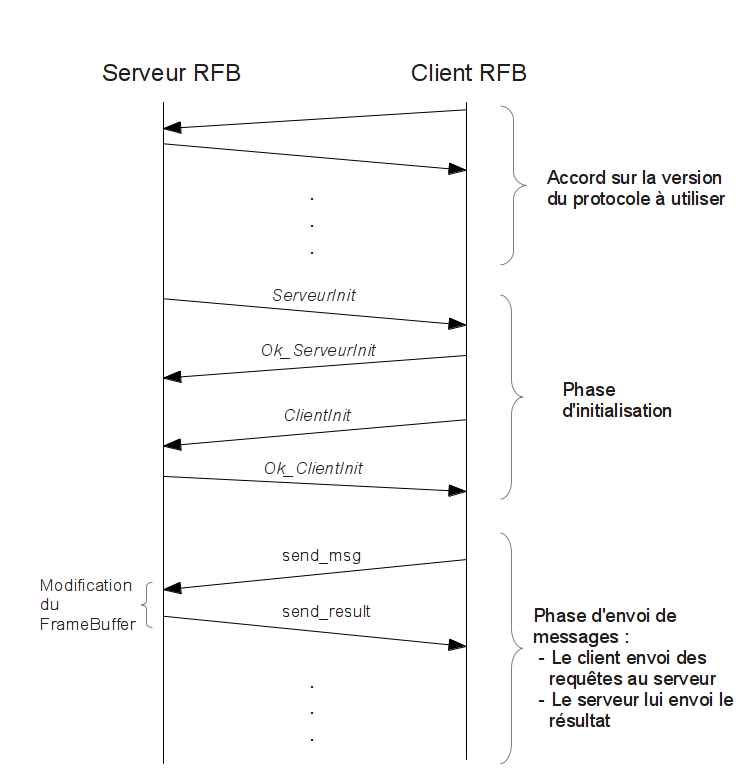
\includegraphics[scale=0.6]{RFBProtocol.png}
		\caption{Communication entre un client RFB et un serveur RFB}
	\end{center}
\end{figure}

\subsection{VNC Côté serveur}

La serveur devra être installé sur la liseuse pour que celle-ci puisse partager son écran. Pour une utilisation optimal, il sera nécessaire de modifier le protocole RFB utilisé par le serveur VNC pour y inclure les événements de la liseuse (événement lors de l'appuie sur une zone de l'écran). Ce serveur va envoyer des directives à DirectFB qui fera ensuite la transition vers le matériel graphique pour modifier l'écran.

\subsection{VNC Côté client}

Un programme client devra pouvoir se connecter au serveur présent sur la liseuse et envoyer des directives pour mettre à jour différentes zones de l'écran de la liseuse.

\begin{figure}[h!]
	\begin{center}
		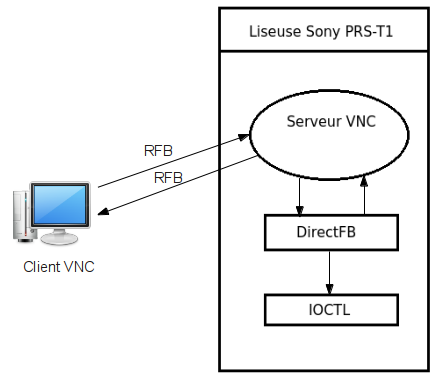
\includegraphics{VNCClientServeur.png}
		\caption{Utilisation de VNC entre la liseuse et un PC hôte}
	\end{center}
\end{figure}

\section{VNC et QEMU}

Un autre point que l'on peut ajouter à ce projet est d'intégrer VNC à QEMU, cela afin que l'émulateur QEMU puisse utiliser le serveur VNC installé sur la liseuse.


\section{Simulateur d'écran}

La dernière étape pour rendre le projet complet est de développer un simulateur d'écran de la liseuse. Pour cela il faut faire en sorte de gérer un affichage cohérent avec les temps de réponse de la liseuse Sony PRS-T1. C'est-à-dire que l'écran doit mettre un certain temps à se rafraîchir et pouvoir modifier seulement certaines zones de l'écran. De plus il faudrait y intégrer la gestion des événements, par exemple lors d'un clique souris simuler un appuie sur une zone de l'écran de la liseuse.

Pour simuler au mieux un écran E-Ink, il faut penser à reproduire la rémanence des anciens affichages. De plus, il faut aussi reproduire la gestion des lookup tables. Cela afin de pouvoir gérer la mise à jour de plusieurs zones de l'écran en simultané.

Enfin, une fois ce simulateur d'écran développé, l'objectif est de l'intégrer à QEMU pour ne plus être dépendant de la liseuse. On aura alors un émulateur complet de la liseuse Sony PRS-T1.
